\part{Features and Capabilities}
The capabilities of Version 0.82 are the following:
\begin{itemize}
\item Audio Impedance Measurement
\item Audio Vector Network Analyzer (Audio Transmission Measurements)
\item Audio Spectrum Analyzer covering up to 40 kHz with graphical display
\item Vector Voltmeter with frequency selectivity and adjustable phase offset
\item Four Signal Generators (added together)  with calibrated output.
\item Weighted and Unweighted Noise Measurement
\item Envelope and Group Delay Measurement
\item Screen Save to BMP file for all functions
\item Calibration of input and output levels and for the touch screen
\item AVNA Control via Serial Port
\end{itemize}

\section{Power Up}When the AVNA is turned on, it starts with an "Audio Test Instrument" screen that allows selection of the function.  This is, as usual, selected by the six touch screen buttons at the bottom of the screen.  In addition, if an $\mu$SD card is present in the Teensy 3.6 socket, a button with "S"  shows in the upper right corner for "Screen Save".

\begin{figure}[H]
\begin{center}
%  \includegraphics[scale=0.75]{zAVNA_Home}
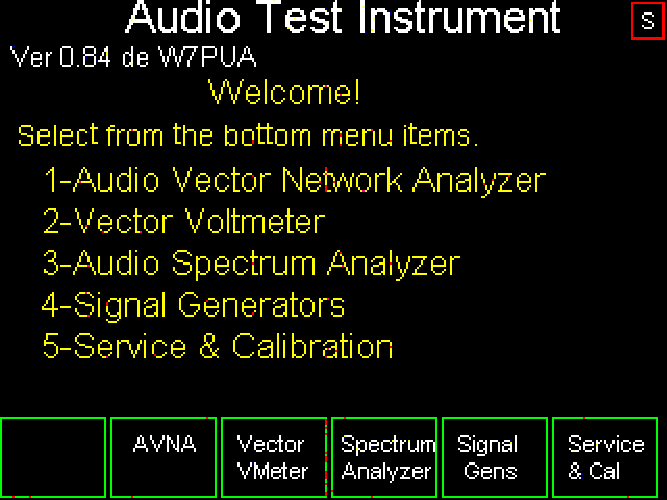
\includegraphics[scale=0.75]{./images/AVNA_000.pdf}
\caption{Power-up Screen}
\label{power-up-label}
\end{center}
\end{figure}

At startup, the Serial Monitor shows the status of the $\mu$SD card followed by a directory listing. For example:
\begin{itemize}
  \item Initializing SD card...and a card is present.
  \item Partition found: FAT32
  \item Volume size (Mbytes): 7378
  \item Files found on the card (name, date, time, and size in bytes):
  \begin{itemize}
   \item AVNA1\_00.BMP  2000-01-01 01:00:00 230454
   \item AVNA1\_01.BMP  2000-01-01 01:00:00 230454
   \end{itemize}
\end{itemize}

\textbf{Note:} $\mu$SD cards have grown in GB capacity over the years.  There may be problems with large capacity cards greater than 8 GB.
